\subsection{\textit{slAdminPlugin}}

La plupart des vues du lot~2 de l'Intranet d'Eyrolles sont générées grâce au plugin Symfony \textit{slAdminPlugin}. Il a été développé en interne par Sensio Labs et est issu de l'abstraction du code d'un précédent projet. Il n'a rien à voir avec la fonctionnalité de génération d'administration intégrée à Symfony. C'est encore un plugin très jeune : Eyrolles est le premier projet qui l'utilise.

\begin{table}
	\centering
	\begin{tabular}{|p{3cm}||p{4.5cm}|p{4.5cm}|}
		\hline
		& Génération d'administration & \textit{slAdminPlugin} \tabularnewline
		\hline
		\hline
		Format de configuration & YAML & code PHP \tabularnewline
		\hline
		Génération de code & oui & non \tabularnewline
		\hline
		Personnalisation de la logique & surcharge de code généré & surcharge de méthodes d'action de base \tabularnewline
		\hline
		Personnalisation des vues & surcharge de \textit{partials} générés & écriture classique de \textit{templates} \tabularnewline
		\hline
	\end{tabular}
	\caption{Comparaison entre la génération d'administration de Symfony et \textit{slAdminPlugin}}
	\label{table:eyrolles_sladmin-vs-admin-gen}
\end{table}

Le tableau~\ref{table:eyrolles_sladmin-vs-admin-gen} reprend une comparaison rapide des différences entre le moteur de génération d'administration de Symfony et \textit{slAdminPlugin}. Le plugin, tout comme la génération d'administration, permet de ne pas avoir à redévelopper la logique des opérations de base, telles que le listing d'éléments, la pagination et le tri de la liste, ou encore la création, l'édition ou la suppression d'éléments. Sa valeur ajoutée est qu'il apporte plus de flexibilité quant à la personnalisation de la logique et des différentes vues.

Un exemple d'implémentation de module utilisant \textit{slAdminPlugin} sera présenté dans la partie~\ref{section:eyrolles_ref-langues}

\textit{slAdminPlugin} s'articule autour de trois composants majeurs :
\begin{itemize}
	\item une classe PHP de configuration ;
	\item des actions d'administration de base ;
	\item des widgets pour agencer la vue.
\end{itemize}

\subsubsection{La classe de configuration}

La classe de configuration permet de stocker les différents paramètres qui seront utilisés pour configurer les actions et la vue d'un module.

Une classe de configuration doit satisfaire les conditions suivantes :
\begin{itemize}
\item elle doit être placée dans le dossier \texttt{lib/config} du module et doit être nommée \texttt{slAdminConfigurationMonNomDeModule};
\item elle doit hériter de la classe abstraite \texttt{slBaseAdminConfiguration} du plugin, qui contient la liste de toutes les options disponibles (cf. Figure~\ref{figure:eyrolles_sladmin-config}) ;
\item la définition des paramètres personnalisés doit se faire dans la méthode \texttt{configure()} surchargée.
\end{itemize}

\begin{figure}
	\centering
	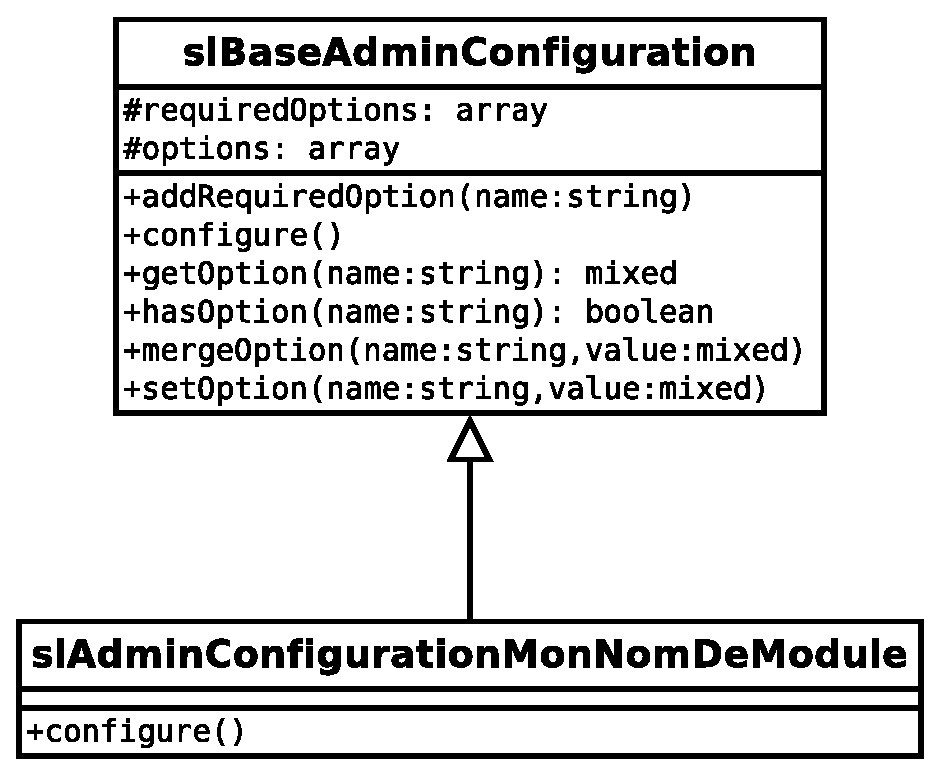
\includegraphics[scale=0.4]{eyrolles_sladmin-config}
	\caption{Classe de configuration de \textit{slAdminPlugin}}
	\label{figure:eyrolles_sladmin-config}
\end{figure}

\subsubsection{Actions de base}

\textit{slAdminPlugin} contient deux classes d'actions qui servent de base aux actions des modules gérés.

La première, \texttt{slBaseActions}, hérite de la classe Symfony \texttt{sfActions}. Elle fournit des méthodes pour gérer les messages de confirmation ou les messages d'erreur, ainsi qu'une méthode de validation de formulaire avancée. La seconde classe, \texttt{slAdminActions}, hérite de \texttt{slBaseActions}. C'est elle qui contient toutes les actions d'administration supportées telles que \texttt{show}, \texttt{list}, \texttt{edit}, \texttt{delete}, \texttt{filter}, \texttt{sort} ou \texttt{batch}.

Ainsi, la classe d'actions d'un module utilisant \textit{slAdminPlugin} doit hériter de la classe \texttt{slAdminActions} au lieu de la classique \texttt{sfActions}. Les méthodes d'action peuvent alors être surchargées si nécessaire.

Ce comportement est décrit dans la Figure~\ref{figure:eyrolles_sladmin-actions}.

\begin{figure}
	\centering
	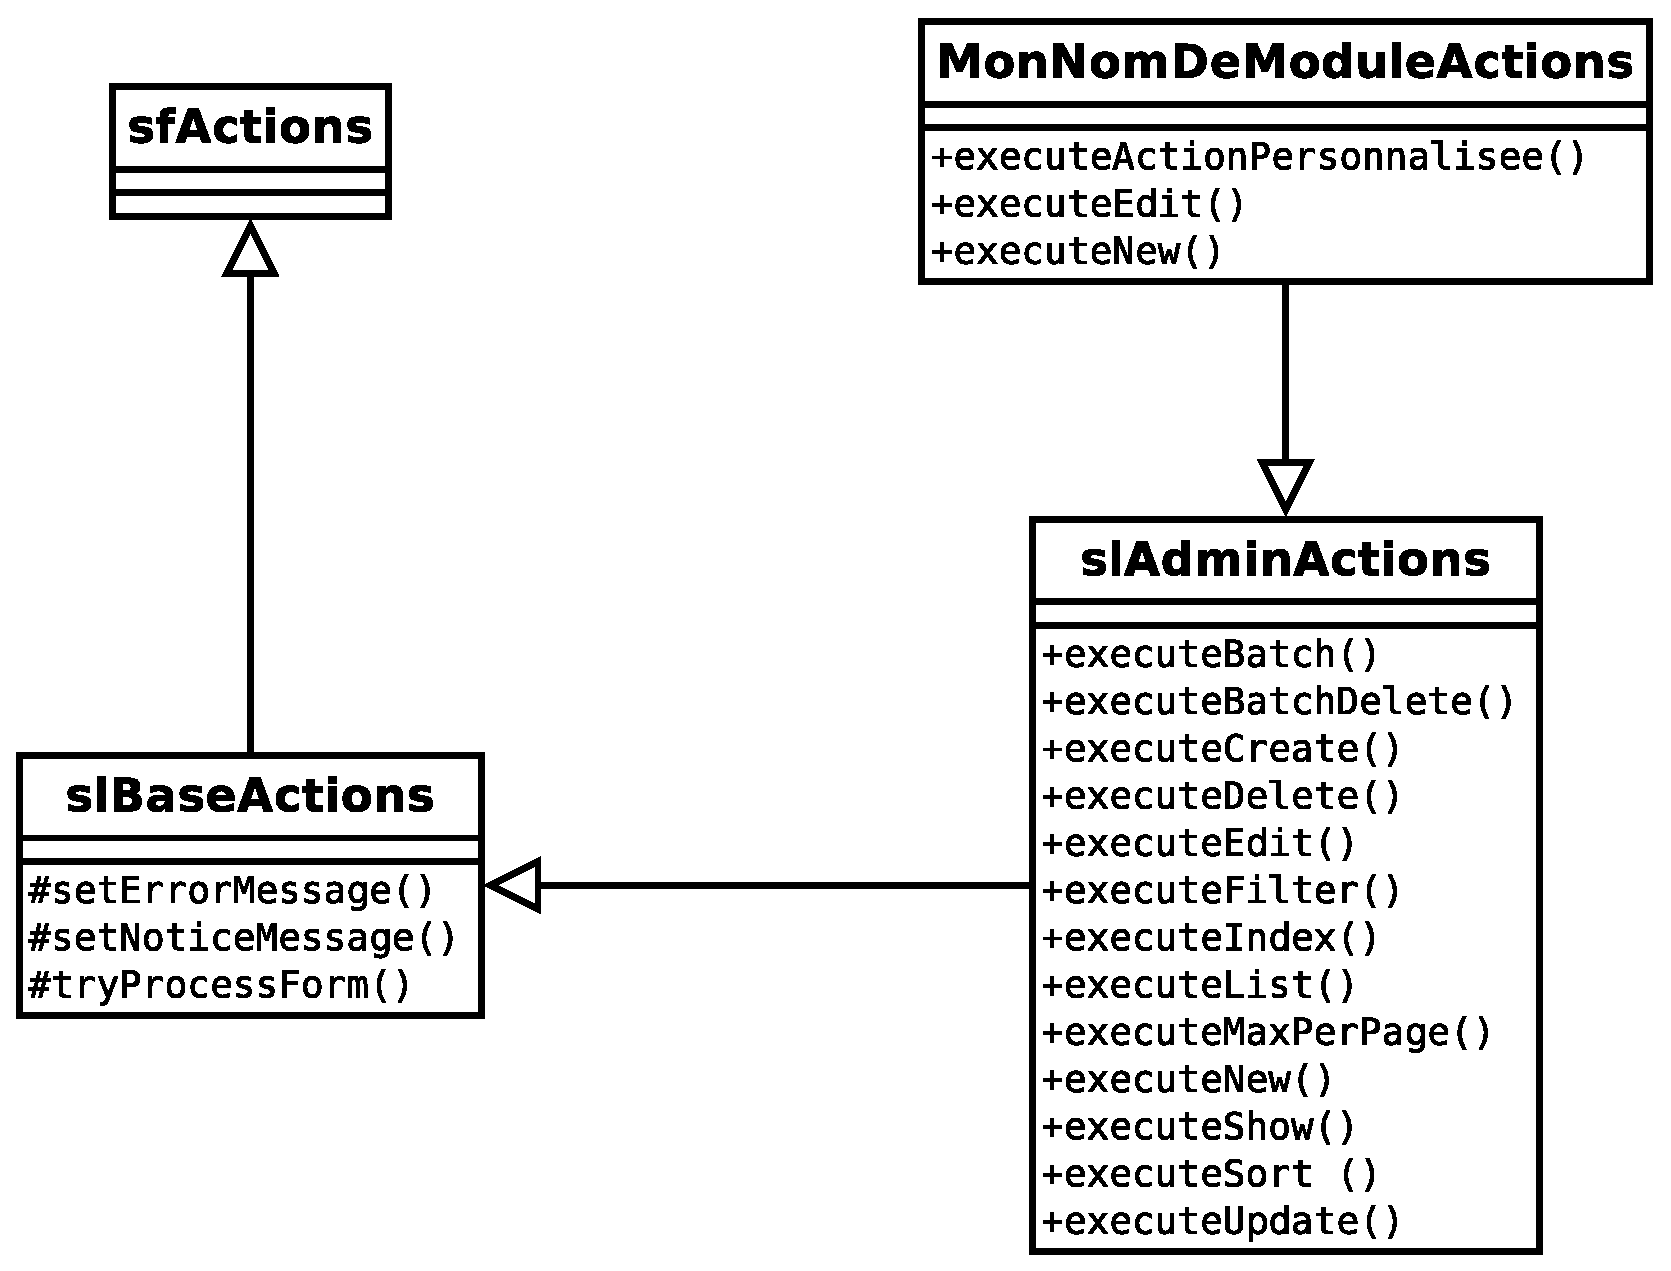
\includegraphics[scale=0.4]{eyrolles_sladmin-actions}
	\caption{Actions de base fournies par \textit{slAdminPlugin}}
	\label{figure:eyrolles_sladmin-actions}
\end{figure}

\subsubsection{Gestion de la vue}

À la base, un module utilisant \textit{slAdminPlugin} doit posséder les cinq \textit{templates} suivants :
\begin{description}
	\item[\texttt{listSuccess.php}] -- le \textit{template} affichant le listing des objets du modèle géré par le module, contenant par exemple les filtres, un tableau d'affichage et un pager ;
	\item[\texttt{listHeader.php}] -- le \textit{partial} affichant la ligne de titre du tableau de listing ;
	\item[\texttt{list\_row.php}] -- le \textit{partial} affichant une ligne du tableau de listing ;
	\item[\texttt{newSuccess.php}] -- le \textit{template} affichant le formulaire de création d'objet ;
	\item[\texttt{editSuccess.php}] -- le \textit{template} affichant le formulaire d'édition d'objet.
\end{description}

Les éléments récurrents de ces vues comme le tableau d'affichage des objets ou le pager sont en réalité des \textit{widgets}, qui sont instanciés dans les actions de base de \textit{slAdminPlugin}. Le nom des classes de ces \textit{widgets} peuvent d'ailleurs être définis dans la classe de configuration du module. Les \textit{widgets} peuvent être affichés dans un \textit{template} comme le montre le Listing~\ref{listing:eyrolles_sladmin-template}.

\lstinputlisting[float, caption={Affichage de \textit{widgets} de \textit{slAdminPlugin} dans un \textit{template}}, label={listing:eyrolles_sladmin-template}]{code/eyrolles_sladmin-template.php}
